\subsection{Product Perspective}
The Students\&Companies (S\&C) platform is a web-based application designed to bridge the gap between university students seeking internships and companies offering them. It serves as a central hub for both parties to connect, collaborate, and manage internship opportunities efficiently. The platform is built around a dynamic matching system that leverages students' profiles, including skills, experiences, and preferences, and pairs them with internships based on the specific needs of the companies.

The platform operates within the broader context of academic institutions, employers, and career services, providing a seamless integration between students’ academic backgrounds and companies’ internship requirements. For companies, S\&C offers tools to post internship opportunities, review applications, and manage the selection process. For students, it facilitates an intuitive search and application process, along with notifications for new internships that match their profile.

Additionally, the platform incorporates a recommendation engine that uses algorithms ranging from simple keyword matching to more sophisticated statistical analyses to ensure the best possible fit between students and internships. By providing an organized environment for companies, students, and universities, the S\&C platform helps streamline the often complex process of internship placement, improving the overall experience for all parties involved. Through feedback systems and monitoring tools, it ensures continuous improvement and responsiveness to user needs. \newline


\subsubsection{Scenarios}
\begin{itemize}
    \item \textbf{Scenario 1 : Signing up and logging in - } User ("S", "C", "U" \footnote{These represent, respectively, an instance of, Student, Company Recruiter, and University Administrator.}) creates an account in the S\&C platform by providing necessary details such as name, email and setting up of password. After successfully completing the registration the user logs in into the platform.
    \item \textbf{Scenario 2 : S creates their profile - } Once logged in, S creates a detailed profile by entering information such as skills, academic grades, relevant experience, and personal details. Additionally, S creates their CV in the platform. The systems gives recommendation to S on writing better CV to ensure the system can better match them with relevant internship opportunities.
    \item \textbf{Scenario 3 : S searches for internships - } S navigates to the search panel within the platform. S enters desired keywords related to job titles, roles, or skills (e.g., "data analysis", "software development", "marketing intern") to find relevant internship openings. The platform uses an intelligent recommendation engine to display internship openings that best match the keywords entered by S. The results are listed in order of the most relevant matches, based on S’s profile data (skills, experience, etc.)
    \item \textbf{Scenario 4 : S applies to internships - } S clicks on a listed internship to open and view the full description. The internship page includes details such as project description, tasks, required skills, company benefits, work conditions (paid/unpaid), and duration. S can also see the company's name and location. S finds an suitable internship and apply directly through the platform by clicking on the "Apply" button. The application is sent to the corresponding company for review containing profile and CV of S.
    \item \textbf{Scenario 5 : C posts an internship - } After logging in the platform, to post an advertisement of an available position of an intern 'C' clicks on the ‘Post a job’ button and then fills out the form regarding the position details like job title, required skills, responsibilities, job location and duration. Once all the details are filled C clicks on the ‘Submit’ button to post it on the platform. After posting C can quickly see a list of all students who are recommended by the system. On clicking of any of the students name C is transferred to the students profile containing the students information and CV. C can also create a questionnaire for the students to answer when their profile is shortlisted.
    \item \textbf{Scenario 6 : C notified of students who have applied - } Whenever any student applies to the position posted by 'C', 'C' is notified instantly in the C\&S platform. On clicking of the students name C is transferred to the students profile containing the students information and CV.
    \item \textbf{Scenario 7 : S\&C matches S and C - } S\&C, the systems gathers information from the key words (skills, experiences) from students' profiles and company's job descriptions and feeds the data to its recommendation model and comes up with a match of S and C. The system then notifies both S and C of this match. Then S and C can either accept or reject the recommendation.
    \item \textbf{Scenario 8 : Selection Process}
    \begin{itemize}
        \item \textbf{Scenario 8.a : C and S both accept S\&C recommendation  - } Once both C and S accept the recommendation a communication channel is opened between them where C can ask for additional information from S. The questionnaire is automatically forwarded by the system to S. S then can fill out the questionnaire and submit. Based on the S's answer C can decide to move forward or not with S.
        \item \textbf{Scenario 8.b : C accepts S's direct application  - } Once C accepts S's application the same process in 8.a happens.
    \end{itemize}
    
    \item \textbf{Scenario 9 : C selects students for interview - } After reviewing the students, C selects those they want to interview and schedules interviews through the platform. Company C uses the platform’s interview scheduling tool to set up a date and time for the interview. The tool integrates with calendar systems to avoid scheduling conflicts. The student receives an email or notification through the platform about the scheduled interview. The notification includes all relevant details such as date, time, and any specific instructions (e.g., virtual meeting link, required documents). C conducts the interview on decided date and time. 

    \item \textbf{Scenario 10 : C finalizes recruitment decision - } After the interview, Company C decides whether to hire or reject S by updating on the S\&C system. The student is notified and it is recorded on the system to be viewed by all the users.
    
    \item \textbf{Scenario 11 : Platform Feedback collects from C and S after interview - } After the selection process finishes S\&C collects feedback from both S and C by asking them to fill out a feedback form and letting it know of any suggestion on how to improve the statical analysis and  recommendation model. Also, C and S will rate the recommendation from 1 to 5 stars.
    
    \item \textbf{Scenario 12 : S\&C Monitors Internship Progress - } Users can  navigate to the monitoring section to view all internship details. S and C can give feedback and raise issues inside the system. U can monitor internship progress of all it's students along with details about the internships they have applied to and their current status (e.g., awaiting interview, accepted, in-progress).

    \item \textbf{Scenario 13 : U handles complaints - } If a student or company raises an issue that requires intervention (e.g., internship termination, disputes), U is notified and takes necessary actions. The decision is then updated in the system and forwarded to students and companies.
\end{itemize}

\subsubsection{Class Diagram}

\begin{figure}[H]
\centering
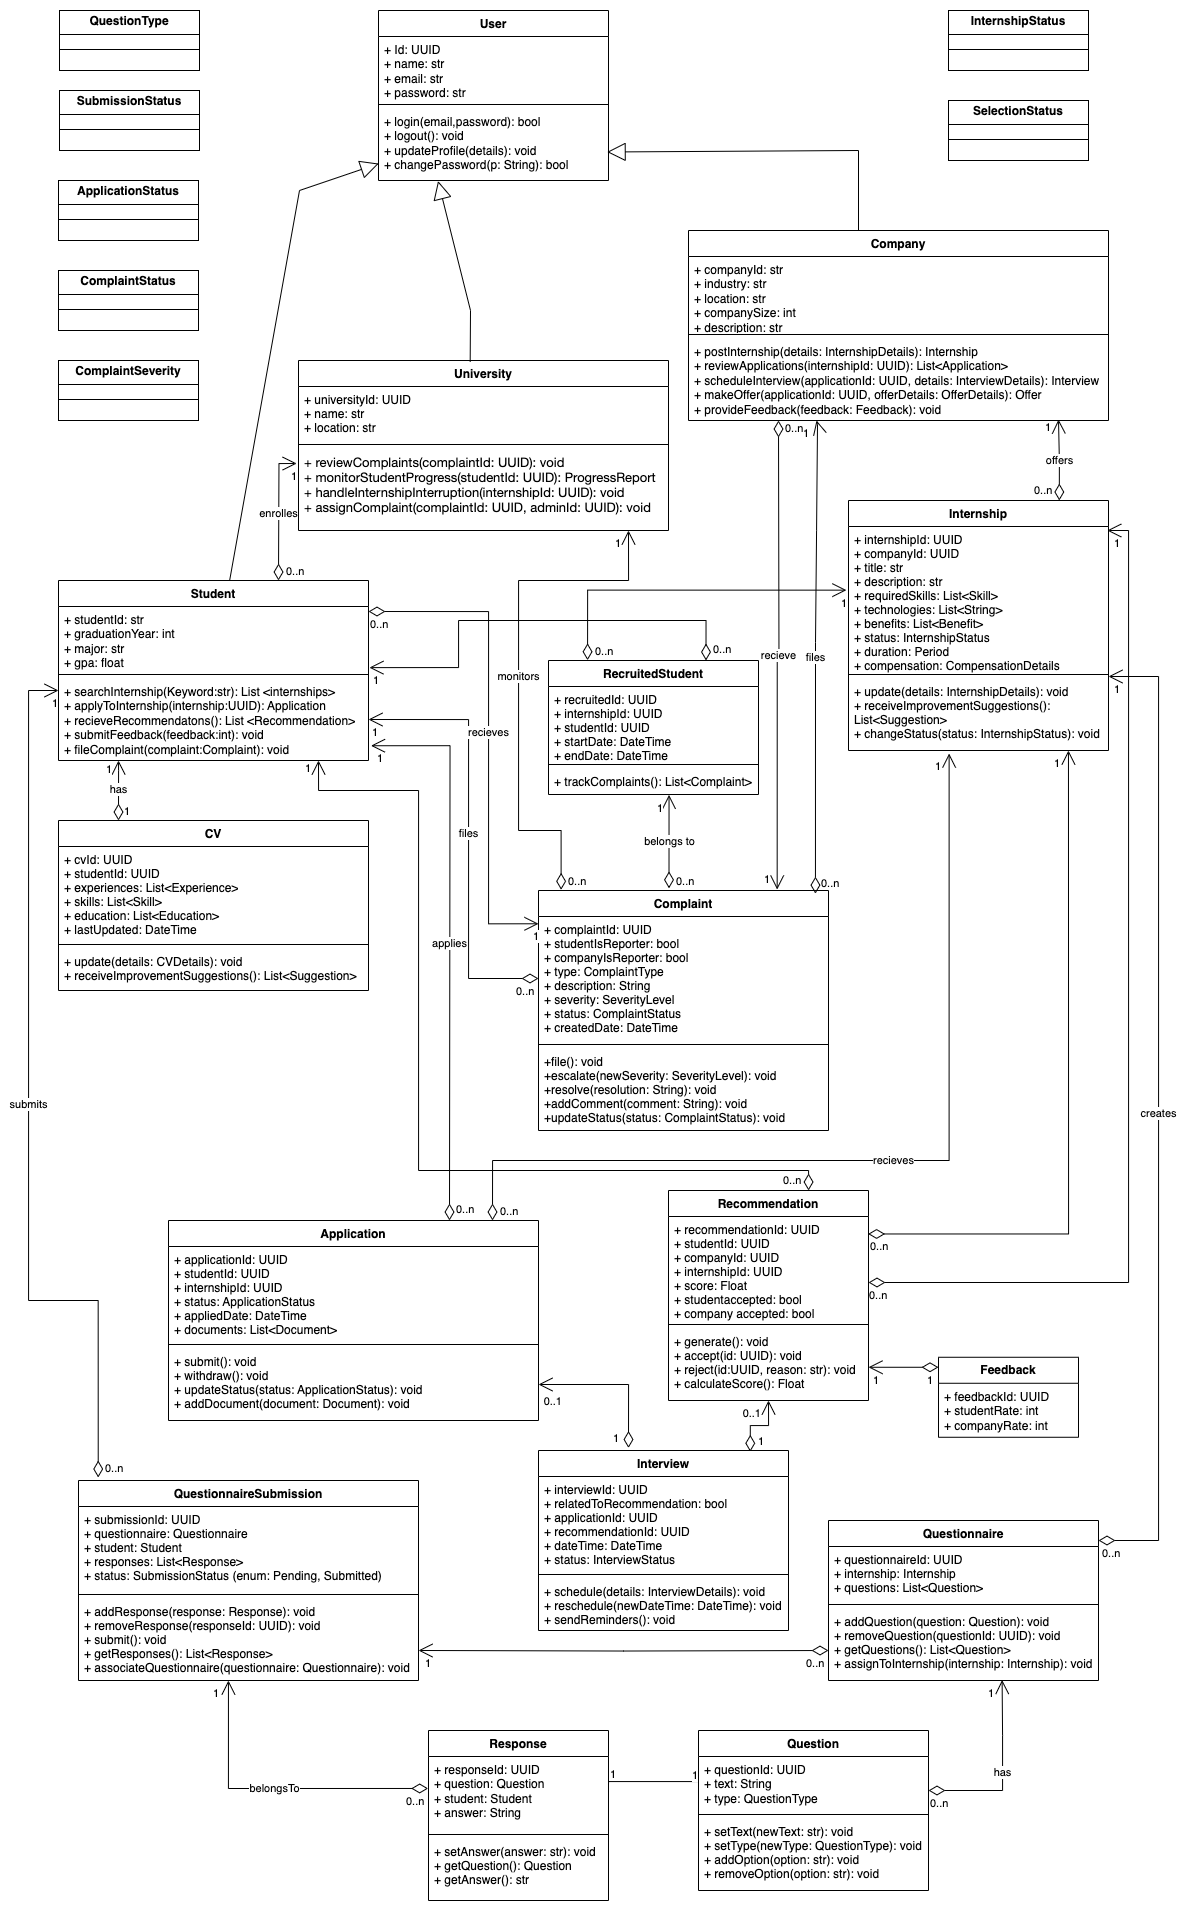
\includegraphics[width=0.8\textwidth]{Images/Class Diagram.drawio (4).png}
\caption{\label{fig:metamodel1}Class Diagram.}
\end{figure}

\subsubsection{State Charts}

In this section we present some state diagrams for the classes that their behavior goes through different states throughout their life cycle.

\begin{figure}[H]
\centering
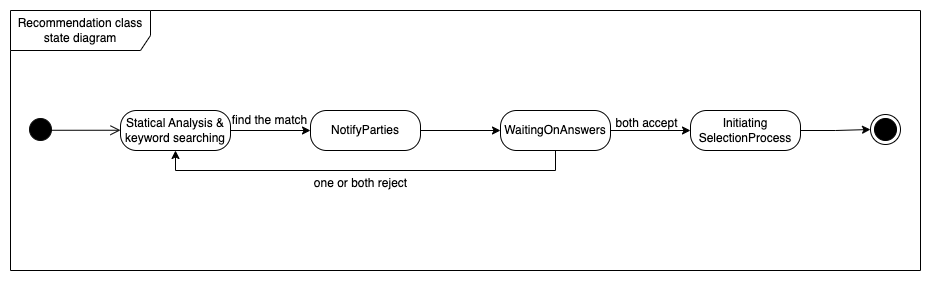
\includegraphics[width=0.8\textwidth]{Images/Recommendation_State_Diagram.drawio.png}
\caption{\label{fig:metamodel1}Recommendation class State Diagram.}
\end{figure}

\begin{figure}[H]
\centering
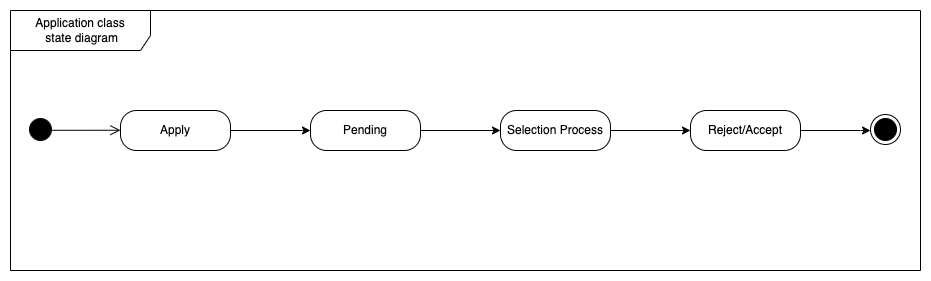
\includegraphics[width=0.8\textwidth]{Images/Application_State_Diagram.drawio.png}
\caption{\label{fig:metamodel1}Application class State Diagram.}
\end{figure}

\begin{figure}[H]
\centering
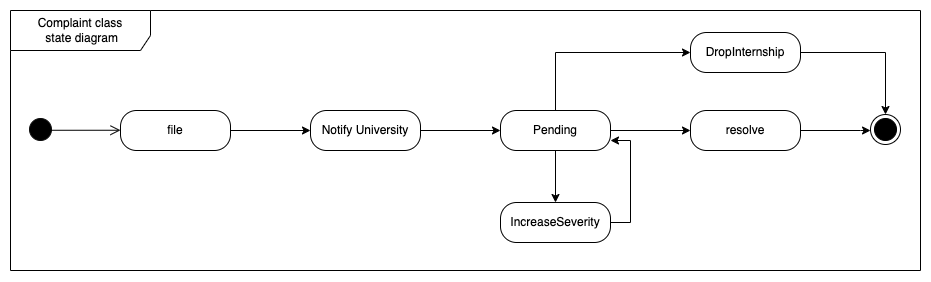
\includegraphics[width=0.8\textwidth]{Images/Complaint_state_Diagram.drawio.png}
\caption{\label{fig:metamodel1}Complaint class State Diagram.}
\end{figure}

\subsection{Product Functions}
The platform C\&S offers several key functions:

\begin{itemize}
    \item \textbf{Student Profile Creation - } Students can create an account, log in, and set up a personalized profile by entering details such as skills, academic background, work experience, and creating their CVs. Recommendations for better CV is given by the C\&S platform.
    \item \textbf{Internship Search \& Application - } Students can search for internships based on various criteria, such as job title, skills required, project domain, location, and internship terms (paid/unpaid, benefits, etc.).The platform presents a list of available internships, ranked according to relevance, and allows students to apply directly through the system.
    \item \textbf{Company Internship Posting - } Companies can post internship opportunities, specifying the project details, required skills, benefits, and terms. Companies can edit, deactivate, or remove internship postings and view applications received from students. Recommendations for better job posting ideas are given by the C\&S platform.
    \item \textbf{Matching Students and Internships - } The systems gathers information from the key words (skills, experiences) from students' profiles and company's job descriptions and feeds the data to its recommendation model and comes up with a match between students and internships. 
    \item \textbf{Selection Process Support - } The platform supports the internship selection process, providing tools to schedule and manage interviews, track application statuses, and maintain communication between students and companies.
    \item \textbf{Interview Scheduling - } Companies can review student applications, shortlist candidates, and schedule interviews (either through integrated video calls or in-person meetings). Companies can use structured questionnaires or direct interviews to assess the suitability of candidates.
    \item \textbf{Feedback \& Evaluation - } After an internship, both students and companies can provide feedback on the internship experience. This feedback is used for improving future recommendations and matching processes. Universities can monitor feedback to ensure academic standards are met and intervene if necessary.
    \item \textbf{Monitoring Progress - } Users can monitors the progress of an internship after the internship has started. Students can Companies can raise complaints.
    \item \textbf{Handling Complaints - } Universities can access a dashboard to track student internship placements, ensure compliance with academic requirements, and mediate any issues or complaints related to internships.

\end{itemize}

\subsubsection{Requirements}
\begin{enumerate}[label=R{\arabic*}]
    \item The S\&C system allows new users (students, universities and companies) to register by giving their credentials (e.g., name, email address, password).
    \item The system allows users (students, universities and companies) to login.
    \item The system allows students to create and update their profile (experience, skills, CV).
    \item The system allows companies to create and update company's profile (about, field of work, achievements).
    \item The system allows universities to create and update their profile.
    \item The system helps students in creating their CVs by giving intelligent suggestion for making a stronger CV and pointing out mistakes.
    \item Students can search for internship opportunities clicking on "Search" button.
    \item Students can apply to desired internship by clicking on "Apply" button for an internship post.
    \item The system provides personalized recommendations to the students for internships based on students profiles and skills which matches with available internships.
    \item Students can automatically apply to any recommended internship by clicking on "Accept" button.
    \item Companies can post internship opportunities and description which includes application domain, tasks to be performed, skills required.
    \item The system can provide recommendations to improve the internship posts by companies.
    \item The companies can prepare a questionnaire in the system to be forwarded to the students to get additional information from them when the selection process starts.
    \item The system can recommend companies about available students who match the job description and skills by applying statical analysis based on the characteristics of students and internships.
    \item The system notifies students and companies once everyday to recommend new matches. 
    \item Companies can track applications and review candidate CVs.
    \item Companies can accept or reject an application or a suggestion by the system by clicking on "Accept" or "Reject" buttons for each application.
    \item A messaging channel is opened when a recommendation is accepted by both student and company or an application by student is accepted by company.
    \item The prepared questionnaire is for forwarded to the student.
    \item The system helps in management of the selection process by scheduling of interview.
    \item The system sends interview link or interview location to both student and company.
    \item The system allows the company to update the interview results.
    \item Interview results are updated in the platform and users are notified.
    \item The system collects feedback from students and companies to then use the gathered data to better its analysis and recommendation algorithm.
    \item The system has a dedicated page to keep track and monitor all the ongoing search and selection processes for all three type of users (students, university, companies).
    \item During the selection process and during interview the involved parties can raise concerns or complains which will be monitored by the university.
    \item The system allows the university to decide on required actions to perform like warning to respective parties or interruption of internship and updates the same on the platform.
\end{enumerate}

\subsection{User Characteristics}
\begin{itemize}
    \item \textbf{Students - }The Students using the Students\&Companies (S\&C) platform are primarily university students. Students familiar with using online platforms for various purposes such as job searching, networking, and academic management. Students create detailed profiles on the platform, including their skills, experiences, and academic achievements, and regularly update their CVs. Their primary goal is to find internship opportunities that align with their academic background, career interests, and personal preferences. They use the platform's search features to explore available internships, apply directly through the system, and receive personalized recommendations based on their profile. Students are proactive in tracking application statuses and attending interviews, and they often seek guidance on improving their CVs and profiles to increase their chances of landing a suitable internship.
    \item \textbf{Companies - }Companies, ranging from small startups to large multinational corporations, use the S\&C platform to find and recruit university interns. The companies have dedicated HR teams who uses different platforms to search for fresh talents. Their main goal is to attract qualified candidates who possess the skills and attitudes needed to contribute to their organizations. Companies post internship opportunities on the platform, specifying the project details, required skills, and benefits offered. They then review student applications, shortlisting candidates for interviews, and use the platform to manage the interview process. Companies rely on the platform’s recommendation system to help identify suitable candidates, and they track the progress of applications and selection procedures.
    \item \textbf{Universities - }Universities play a critical role in overseeing student internships. University administrators and career service staff use the S\&C platform to track and manage student internship placements. Universities use the platform to ensure that internships meet academic standards and address any issues that may arise during the internship period. In case of disputes or complaints, universities mediate between students and companies to ensure that both parties fulfill their commitments.
\end{itemize}

\subsection{Domain Assumptions}
\begin{enumerate}[label=D{\arabic*}]
\item Users have working internet connection.
\item Student profiles are accurate and up-to-date.
\item Internship availability is regularly updated.
\item Internship descriptions are clear and comprehensive.
\item Details provided by students and companies are true.
\item Student's eligibility for an internship is supervised by university.
\item Students and companies select their available times correctly during interview setup procedure.
\item During complaint resolution process parties actually resolve the conflict.
\end{enumerate}

\subsection{Dependencies}

For the registration process, a verification email must be sent by the system through to let Users successfully
sign up, thus requiring the integration of an EmailService. Also during interview scheduling EmailService is used to notify students.



